\iffalse
\bibliography{reference/refs}
\fi


\chapter{Foundamental theory}
\label{chap:foundamental}

The rest of this thesis would introduce our own approaches of face de-identification
for images and videos. Therefore, some foundamental theories need to be explained in
advance. In this section, we introduce the concepts of tensor and active apearance model.

To distinguish from scalars, vectors, matrices and higher-order tensors, kinds of 
symbols are used. Scalars are represented by Greek alphabet letters and low case letters $\alpha,\beta,
\lambda,...,a,b,c,...$. Vectors are denoted by bold lower case letter ${\bf (a,b,c,...)}$. Matrices are
shown as $(A,B,C,...)$. Tensors are described by calligraphic letters $(\mathcal{A,B,C,...})$. 
A tensor of order $n$ is denoted by $\mathcal{A} \in R^{i_1 \times i_2 \times ... \times i_n}$, where $n$ 
is the order. $\mathcal{A}$ can be flattened to a matrix by stacking its mode-$m$ vectors as columns: 
$A_{(m)} \in R^{i_m \times (i_1i_2...i_{m-1}i_{m+1}...i_n)}$. 



\section{Tensor}

Tensor is the generalized form of scalar, vector and matrix. 
Formally, tensor is the $N$-order array. For example, $1$-order 
tensor is vector and $2$-order tensor is matrix. The higher-order 
tensor ($N > 3$) is a multidimensional array. For any $N$ 
dimensional tensor, it could be unfolded to a matrix.
Figure \ref{fig:tensor_fold} shows an unfolding example for a $3$-order tensor.

	\begin{figure}[!htb]
	    \centering
	    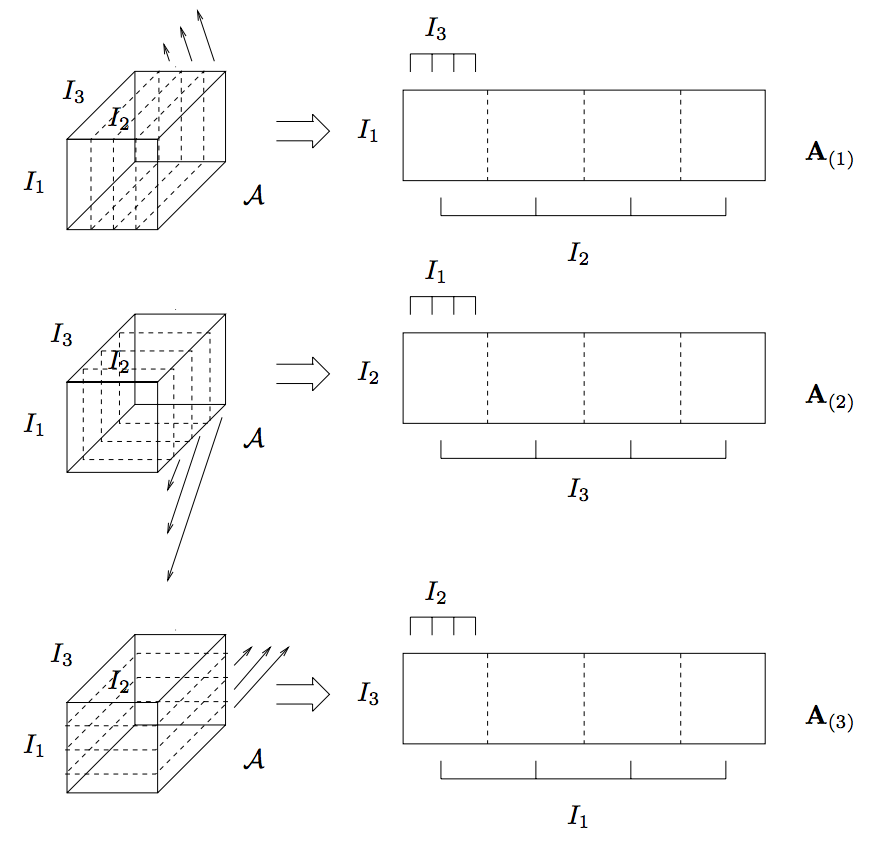
\includegraphics[scale=0.9]{figure/tensor_definition}
	    \caption{Tensor unfolding example. The tensor is $\mathcal{A} \in R^{I_1 \times I_2 \times I_3}$.
	    		The unfolded matrixes are $A_1 \in R^{I_1 \times I_2I_3}$, $A_2 \in R^{I_2 \times I_1I_3}$
	    		and $A_3 \in R^{I_3 \times I_1I_2}$.}
	    \label{fig:tensor_fold}
	\end{figure}

In mathematical, a $(r+s)$-order tensor is a set of scalars 
in $(r+s)$ dimensions and it is represented as:

	\begin{equation}
	\label{equ:tensor}
	      \begin{aligned}
	        \mathcal{A} = a_{i_1i_2...i_r}^{j_1j_2...j_s},
	      \end{aligned}
    \end{equation}
	where $a_{i_1i_2...i_r}^{j_1j_2...j_s}$ is one of the items.
	We think that a higher-order tensor is an arrangement of
	data items. We can find the relations between the data items
	by analyzing the constructed tensor.

\subsection{Higher-Order Singular Value Decomposition}

	Generally, an object is indicated as a vector. For example,
	a 3D point, ${\bf a} \in R^{3}$, is shown as ${\bf a} = [x,y,z]$.
	In face image processing, each item is represented as a vector. 
	With each row as an item, the face images are constructed as a 
	matrix. The PCA could extract the
	principle component of the data \cite{EigenFace91,EigenFace97}, which would
	find out the most significant common factor among the data.
	For the data containing two types of variations, a bilinear 
	model could be used to extract the factors individually based
	on SVD \cite{Bilinear97,Bilinear00,Bilinear04}.
	Similarly, the enough images can be built up as a higher-order
	tensor. The parameters for each dimension is extracted through HOSVD.

	According to the HOSVD \cite{Lathauwer00,Lathauwer_rank}, any 
	tensor $\mathcal{C} \in R^{i_1 \times i_2 \times ... \times 
	i_n}$ could be decomposed as:
	\begin{align}
		\label{equ:hosvd}
		\begin{split}
			\mathcal{C} = \mathcal{C}_{core} \times_1 U_1 \times_2 U_2 ... \times_n U_n,
		\end{split}
	\end{align}
	where $\mathcal{C}_{core}$ is a core tensor whose size is the same as $\mathcal{C}$, $U_i$ is the left part in SVD results 
	of corresponding mode-$i$ flattening of $\mathcal{C}$.

	\subsection{CP Decomposition}
	There are many other tensor decomposition approaches such as CANDELINC, 
	PARAFAC2 \cite{Candelinc80,Parafac72}. Aiming at decomposing a parameter
	entity into factors of each dimension, the CP decomposition is applied
	in this thesis.
	Firstly introduced in \cite{CP27,CP27_2},
	the tensor CP decomposition assumes that any 
    tensor can be represented as a sum of the tensor product by rank-one tensors.
    \cite{Lathauwer_rank}, shown as (\ref{equ:cp}).

    \begin{equation}
	      \label{equ:cp}
	      \begin{aligned}
	        \mathcal{C} = \sum_{i=1}^{r}\lambda_i * {\bf c_1^i} \circ {\bf c_2^i} \circ...\circ {\bf c_n^i},  
	      \end{aligned}
    \end{equation}
    where $\circ$ indicates tensor product. It indicates that $\mathcal{C} \in R^{i_1 \times i_2 \times ... \times i_n}$ 
    can be decomposed into $r$ components of tensor product by $n$ vectors.

    \begin{figure}[!htb]
	    \centering
	    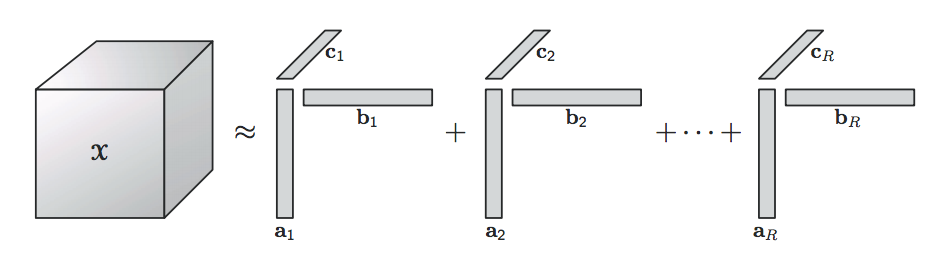
\includegraphics[scale=0.9]{figure/CP_Decomposition}
	    \caption{The CP decomposition of a $3$-order tensor. }
	    \label{fig:cp_de}
	\end{figure}

	Figure \ref{fig:cp_de} illustrates the CP decomposition of a $3$-order tensor.
	It is a rank-$r$ decomposition which means the tensor $\mathcal{X}$ is estimated
	by the sum of $r$ outer product by $a_i,b_i,c_i$.


\section{Active Appearance Model}
	
	Inteprating a face image with statistical models is a general solution to
	image representation. The Snake \cite{Snake88} and ASM \cite{ASM95} are
	used to find face boundary so that the landmarks are located. Considering
	the appearance, AAM \cite{AAM98,AAM01,Matthews_04} inteprates the face
	image in two aspects: shape and appearance. The figure \ref{fig:aam} is
	the AAM instance for one face image.

	\begin{figure}[!htb]
	    \centering
	    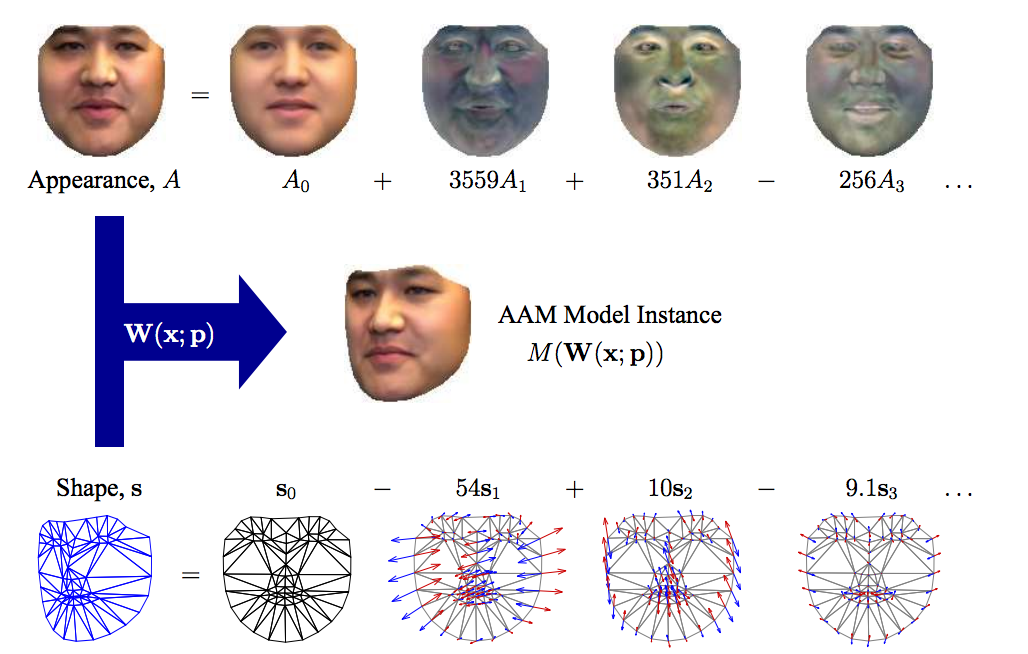
\includegraphics[scale=0.82]{figure/aam}
	    \caption{An AAM instance. The appearance and shape are deformed individually
	    by altering the coefficients and the appearance is warped to the shape at last.}
	    \label{fig:aam}
	\end{figure}

	The shape of a face is represented as the coordinates set of $n$ landmarks ${\bf s} = 
	\{x_1,x_2,...,x_n,y_1,y_2,...,y_n\}$. The appearance is the set of pixels (the total number
	is $m$) within face shape $A=\{p_1,p_2,...,p_m\}$. In statistical models, all sample images
	are gathered to get parameters representation. 

	For shapes,
	\begin{align}
		\label{equ:aam_shape}
		\begin{split}
			{\bf s} = {\bf s_0} + \sum_{i=1}^{n}\gamma_i * {\bf s_i},
		\end{split}
	\end{align}
	where ${\bf s_0}$ is the mean appearance of sample images, ${\bf s_i}$ is the PCA 
	component of shapes and $\gamma_i$ is the coefficient for each component. 

	Similarly, the appearance statistical model is:
	\begin{align}
		\label{equ:aam_appearance}
		\begin{split}
			A = A_0 + \sum_{i=1}^{n}\lambda_i * A_i,
		\end{split}
	\end{align}
	where $A_0$ is the mean appearance of sample images, $A_i$ is the PCA component 
	of appearances and $\lambda_i$ is the corresponding coefficient. 

	The AAM is widely used in landmarks detection \cite{landmarks14}, face recognition
	\cite{aamFR98}, expression recognition \cite{aamER09}, expression transfer \cite{Theobald07}, etc.
